%%%%%%%%%%%%%%%%%%%%%%%%%
% Dokumentinformationen %
%%%%%%%%%%%%%%%%%%%%%%%%%
\newcommand{\titleinfo}{Robotik - Formelsammlung}
\newcommand{\authorinfo}{Silvano Ferretti, Sven Arnold, Arjen Visser}
\newcommand{\versioninfo}{$Revision: 0 $ - powered by \LaTeX}

%%%%%%%%%%%%%%%%%%%%%%%%%%%%%%%%%%%%%%%%%%%%%
% Standard projekt�bergreifender Header f�r
% - Makros 
% - Farben
% - Mathematische Operatoren 
%
% DORT NUR ERG�NZEN, NICHTS L�SCHEN
%%%%%%%%%%%%%%%%%%%%%%%%%%%%%%%%%%%%%%%%%%%%%  
%BuG-Fix
%Package pdf Error: Driver file ................ not found
%If you have a luatex driver fail uncomment these lines
%\RequirePackage{luatex85}
%\def\pgfsysdriver{pgfsys-pdftex.def}

% Genereller Header
\documentclass[11pt,twoside,a4paper,fleqn]{article}
% Dateiencoding
\usepackage[utf8]{inputenc}
\usepackage[T1]{fontenc}	%ä,ü...
% Seitenränder
\usepackage[left=1cm,right=1cm,top=0.5cm,bottom=0.2cm,includeheadfoot]{geometry}
\setlength{\headsep}{5pt} 
% Sprachpaket
\usepackage[english, ngerman]{babel} % Silbentrennung und Rechtschreibung Englisch und Deutsch

%%%%%%%%%%%%%%%%%%%%%%%
%% Wichtige Packages %%
%%%%%%%%%%%%%%%%%%%%%%%

\usepackage{amsmath}                % Allgemeine Matheumgebungen									
\usepackage{amssymb}                % Fonts: msam,msbm, eufm & Mathesymbole, Mengen (lädt automatisch amsfonts)									
\usepackage{array}                  % \newcolumntype, \firsthline, ,\lasthline, m{width}, b{width}									
\usepackage{caption}                % Bildunterschriften									
\usepackage{enumitem}               % basic environments: enumerate, itemize, description									
\usepackage{fancybox}               % \fbox: \shad­ow­box, \dou­ble­box, \oval­box, \Oval­box									
\usepackage{fancyhdr}               % Seiten schöner gestalten, insbesondere Kopf- und Fußzeile									
\usepackage{floatflt}               % Textumflossene Abbildungen \begin{floatingfigure}[r]{Breite} : r rechts, l links, p links auf geraden Seiten und rechts auf ungeraden Seiten									
\usepackage{graphicx}               % \includegraphics[keyvals]{imagefile}, [draft]graphicx zeigt nur Namen und Rahmen an, [final] hebt diese option auf => Bild wird angezeigt    									
\usepackage{hyperref}               % Erstellt Verweise innerhalb und nach außerhalb eines PDF Dokumentes.								
\usepackage{lastpage}               % Bspw. : Page 1 of 3 => \thepage\ of \pageref{LastPage}									
\usepackage{listings}               % Erlaubt es Programmcode in der gewünschten Sprache zu hinterlegen (C++, Matlab,..). Definition der Sprache mit \lstset{language=name}..									
\usepackage{longtable}              % Longtable erlaubt es Tabellen zu erstellen die bei der nächsten Seite weiterlaufen. (Bricht automatisch um)									
\usepackage{mathabx}                % Mathesymbole									
\usepackage{mathrsfs}               % \mathscr (Benötigt für Fourierreihen-Symbol)									
%\usepackage{mathtools}              % Extension package to amsmath									
\usepackage{multicol}               % multicols-Umgebung \begin{multicols}{3} erzeugt Abschnitt mit 3 Spalten									
\usepackage{multirow}               % Tabelle: ermöglicht es Felder mehrerer Zeilen in einem zusammenzufassen									
\usepackage{pdflscape}              % adds PDF support to the environment 'landscape'									
\usepackage{pxfonts}                % Symbole, griechisches Alphabet, Integrale...									
\usepackage{rotating}               % sideways, turn{degree}, rotate{degree}, sidewaysfigure, sidewaystable Umgebung									
\usepackage{subcaption}             % Bildunterschriften für Subfigures									
\usepackage{tabularx}               % tabularx-Umgebung: Hat feste Gesamtbreite, \begin{tabularx}{\textwidth}{c c c c c} X: Spalte mit variabler Breite, l, c, r, p{breite}, m{breite}									
\usepackage{textcomp}               % text symbols: baht, bullet, copyright, musical-note, onequarter, section, yen									
\usepackage{tikz}                   % Tikz Umgebung zur Grafikerzeugung									
\usepackage{titlesec}               % Überschriften zu Textabstände
\usepackage{trfsigns}               % Transformationszeichen \laplace, \Laplace..									
\usepackage{trsym}                  % Weitere Laplace Zeichen erlaubt auch vertikale Transformationszeichen									
\usepackage{verbatim}               % verbatim, verbatim*, comment Umgebung									
\usepackage{wrapfig}                % Textumflossene Bilder und Tabellen, \begin{wrapfigure}[Zeilen]{Position}[Ueberhang]{Breite}									
\usepackage{xcolor}                 % \pagecolor{color}, \textcolor{color}{text}, \colorbox{color}{text}, \fcolorbox{border-color}{fill-color}{text}									
\usepackage{titlesec}
% Zum Bilder einfach in Tabellen einfügen (valign=t)
\usepackage[export]{adjustbox}

%%%%%%%%%%%%%%%%%%%%
% Generelle Makros %
%%%%%%%%%%%%%%%%%%%%
\newcommand{\skript}[1]{$_{\textcolor{red}{\mbox{\small{Skript S.#1}}}}$}
\newcommand{\verweis}[2]{\small{(siehe auch \ref{#1}, #2 (S. \pageref{#1}))}}
\newcommand{\verweiskurz}[1]{(\small{siehe \ref{#1}\normalsize)}}
\newcommand{\subsubadd}[1]{\textcolor{black}{\mbox{#1}}}
\newcommand{\formelbuch}[1]{$_{\textcolor{red}{\mbox{\small{S#1}}}}$}

\newcommand{\robos}[1]{$_{\textcolor{red}{\mbox{\small{Ind.Rob S. #1}}}}$}
\newcommand{\robo}[2]{$_{\textcolor{red}{\mbox{\small{Ind.Rob S. #1 K. #2}}}}$}
\newcommand{\stoecker}[1]{$_{\textcolor{grey}{\mbox{\small{Stöcker #1}}}}$}
\newcommand{\sachs}[1]{$_{\textcolor{blue}{\mbox{\small{Sachs S. #1}}}}$}
\newcommand{\hartl}[1]{$_{\textcolor{green}{\mbox{\small{Hartl S. #1}}}}$}

\newcommand{\schaum}[1]{\tiny Schaum S. #1}

\newcommand{\skriptsection}[2]{\section{#1 {\tiny Skript S. #2}}}
\newcommand{\skriptsubsection}[2]{\subsection{#1 {\tiny Skript S. #2}}}
\newcommand{\skriptsubsubsection}[2]{\subsubsection{#1 {\tiny Skript S. #2}}}

\newcommand{\matlab}[1]{\footnotesize{(Matlab: \texttt{#1})}\normalsize{}}

% Syntax: \bmu{Pfad zum Bild}{Bildgrösse}{Beschriftung des Bildes}
\newcommand{\bl}[2]{
	\begin{figure}[h]
		\flushleft  % linksbuendig
		\includegraphics[width=#1]{#2} \\
	\end{figure}
}
\newcommand{\br}[2]{
	\begin{figure}[h]
		\flushright  % rechtsbuendig
		\includegraphics[width=#1]{#2} \\
	\end{figure}
}

\newcommand{\bild}[2]{
	\begin{figure}[h]
		\centering  % zentriert
		\includegraphics[width=#1]{#2} \\
	\end{figure}
}

\newcommand\tabbild[2][]{%
	\raisebox{0pt}[\dimexpr\totalheight+\dp\strutbox\relax][\dp\strutbox]{%
		\includegraphics[#1]{#2}%
	}%
}

\newcolumntype{P}[1]{>{\raggedright\arraybackslash}p{#1}} %Tabelle linksausgerichtet
\newcolumntype{L}[1]{>{\raggedleft\arraybackslash}p{#1}} %Tabelle rechtsausgerichtet
\newcolumntype{C}[1]{>{\centering\arraybackslash}p{#1}}


\setitemize{noitemsep,topsep=0pt,parsep=0pt,partopsep=0pt} %kompakte itemize
\setenumerate{noitemsep,topsep=0pt,parsep=0pt,partopsep=0pt} %kompakte enumerate

%%%%%%%%%%
% Farben %
%%%%%%%%%%
\definecolor{black}{rgb}{0,0,0}
\definecolor{red}{rgb}{1,0,0}
\definecolor{white}{rgb}{1,1,1}
\definecolor{grey}{rgb}{0.8,0.8,0.8}
\definecolor{green}{rgb}{0,.8,0.05}
\definecolor{brown}{rgb}{0.603,0,0}
\definecolor{mymauve}{rgb}{0.58,0,0.82}


%%%%%%%%%%%%%%%%%%%%%%%%%%%%
% Mathematische Operatoren %
%%%%%%%%%%%%%%%%%%%%%%%%%%%%
\DeclareMathOperator{\sinc}{sinc}
\DeclareMathOperator{\sgn}{sgn}
\DeclareMathOperator{\Real}{Re}
\DeclareMathOperator{\Imag}{Im}
%\DeclareMathOperator{\e}{e}
\DeclareMathOperator{\cov}{cov}
\DeclareMathOperator{\PolyGrad}{PolyGrad}

%Grösse Integral anpassen
\def\Int{\mbox{\Large$\displaystyle\int$\normalsize}}
\def\OInt{\mbox{\Large$\displaystyle\oint$\normalsize}}

%Makro für 'd' von Integral- und Differentialgleichungen 
\newcommand*{\diff}{\mathop{}\!\mathrm{d}}

%%%%%%%%%%%%%%%%%%%%%%%%%%%
% Fouriertransformationen %
%%%%%%%%%%%%%%%%%%%%%%%%%%%

% Fouriertransformationen
\unitlength1cm
\newcommand{\FT}
{
	\begin{picture}(1,0.5)
	\put(0.2,0.1){\circle{0.14}}\put(0.27,0.1){\line(1,0){0.5}}\put(0.77,0.1){\circle*{0.14}}
	\end{picture}
}


\newcommand{\IFT}
{
	\begin{picture}(1,0.5)
	\put(0.2,0.1){\circle*{0.14}}\put(0.27,0.1){\line(1,0){0.45}}\put(0.77,0.1){\circle{0.14}}
	\end{picture}
}


%%%%%%%%%%%%%%%%%%%%%%%%%%%%
% Allgemeine Einstellungen %
%%%%%%%%%%%%%%%%%%%%%%%%%%%%

%Pdf Info
\hypersetup{pdfauthor={\authorname},pdftitle={\titleinfo},colorlinks=false}
\author{\authorname}
\title{\titleinfo}

% Abstände Text zu Übertiteln / Einzug
\titlespacing{\section}{12pt}{1em}{0.5em}
\titlespacing{\subsection}{12pt}{1em}{0.5em}
\titlespacing{\subsubsection}{12pt}{1em}{0.5em}

%%%%%%%%%%%%%%%%%%%%%%%
% Kopf- und Fusszeile %
%%%%%%%%%%%%%%%%%%%%%%%
\pagestyle{fancy}
\fancyhf{}
%Linien oben und unten
\renewcommand{\headrulewidth}{0.5pt} 
\renewcommand{\footrulewidth}{0.5pt}

%Kopfzeile links bzw innen
\fancyhead[L]{\titleinfo{ }}
%Kopfzeile mitte
%\fancyhead[C]{}
%Kopfzeile rechts bzw. aussen
\fancyhead[R]{Seite \thepage { }von \pageref{LastPage}}

%Fusszeile links bzw. innen
\fancyfoot[L]{\footnotesize{\authorname}}
%Fusszeile mitte
%\fancyfoot[C]{\footnotesize{\authoremail}}
%Fusszeile rechts bzw. ausen
\fancyfoot[R]{\footnotesize{\today}}
% Einrücken verhindern versuchen
\setlength{\parindent}{0pt}

%%%%%%%%%%%%%%%%%%%%%%%%%%%%%%%%%%%%%%%
%% Makros & anderer Low-Level bastel %%
%%%%%%%%%%%%%%%%%%%%%%%%%%%%%%%%%%%%%%%
% Zeilenhöhe Tabellen:
\newcommand{\arraystretchOriginal}{1.5}
\renewcommand{\arraystretch}{\arraystretchOriginal}

\makeatletter
%% Makros für den Arraystretch (bei uns meist in Tabellen genutzt, welche Formeln enthalten)
% Default Value
\def\@ArrayStretchDefault{1} % Entspricht der Voreinstellung von Latex

% Setzt einen neuen Wert für den arraystretch
\newcommand{\setArrayStretch}[1]{\renewcommand{\arraystretch}{#1}}

% Setzt den arraystretch zurück auf den default wert
\newcommand{\resetArrayStretch}{\renewcommand{\arraystretch}{\@ArrayStretchDefault}}

% Makro zum setzten des Default arraystretch. Kann nur in der Präambel verwendet werden.
\newcommand{\setDefaultArrayStretch}[1]{%
    \AtBeginDocument{%
        \def\@ArrayStretchDefault{#1}
        \renewcommand{\arraystretch}{#1}
    }
}
\makeatother

%% Achtung Symbol \danger
\newcommand*{\TakeFourierOrnament}[1]{{%
        \fontencoding{U}\fontfamily{futs}\selectfont\char#1}}
\newcommand*{\danger}{\TakeFourierOrnament{66}}

% M�glichst keine Erg�nzungen hier, sondern in header.tex
\begin{document} 
%%%%%%%%%%%%%%%%%%%%%%%%%%%%%%%%%%%%%%%%%%%%%%%%%%%%%%%%%%%%%%%%%%%%%%%%%%%%%%%%%%%%%%%%%%%%%%%
%%%%%%%%%%%%%%%%%%%%%%%%%%%%%%%%%%%%%%%%%%%%%%%%%%%%%%%%%%%%%%%%%%%%%%%%%%%%%%%%%%%%%%%%%%%%%%%
\section{Mathematische Grundlagen der Robotik}

	\subsection{TI Taschenrechner Befehle}
\begin{tabular}{p{5cm}p{10cm}}

\texttt{$[ x_{11} , x_{12} ; x_{21},x_{22}]$} &  $ \begin{bmatrix}
            	x_{11} & x_{12}\\
            	x_{21} & x_{22}\\
            \end{bmatrix} $ \\
\texttt{ $[ \ldots]^{-1} $} & Inverse Matrix\\
\texttt{ $[ \ldots] $ (2ND CATALOG) \small{T} } & Transponierte Matrix
$[\ldots]^{T}$\\

\end{tabular} \\
	

	\subsection{Matritzenrechnen}
		\subsubsection{Vektoren im Raum}
			$\vec{p}_{AB}=
			\begin{matrix}
            	x_B-x_A\\
            	y_B-y_A\\
            	z_B-z_A\\
            \end{matrix}$\\
			
			Transponierung: $a^T\cdot b= \left(a_1 \vspace{0.2cm} a_2\vspace{0.2cm}  \ldots a_n \right) 
			\cdot $
	
		\subsubsection{Matrizen Multiplikation \small{(A muss gleich viele Spalten
		haben wie B Zeilen hat)}}
		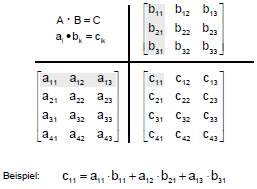
\includegraphics[width=7cm]{./bilder/matrizenmultiplikation.png}
    	
	
	
	
\subsection{Übersicht}
	\begin{tabular}{l l}
    	Transponierte Matrix: & $A^T=[a_{ik}^T]=[a_{ki}]$ vertauschen der Zeilen
    	mit Spalten\\
    	Einheitsmatrix:& $I_n= 
			    	\begin{bmatrix} 
			        	1&0 & 0\\
			        	0&1&0\\
			        	0&0&1                               
			        \end{bmatrix}$		    
    \end{tabular}

\subsection{Determinante}

	\textbf{2x2 Matrix}    
	$$ \det \begin{bmatrix} a_{11} & a_{12} \\ a_{21} & a_{22} \end{bmatrix} =
	a_{11} a_{22} - a_{12} a_{21}.  $$
	
	\textbf{3x3 Matrix}
	$$ \det \begin{bmatrix} a_{11} & a_{12} & a_{13} \\ a_{21} & a_{22}& a_{23} \\
	a_{31} & a_{32} & a_{33} \end{bmatrix} \\ = a_{11} a_{22} a_{33} + a_{12}
	a_{23} a_{31} + a_{13} a_{21} a_{32} - a_{13} a_{22} a_{31} - a_{12} a_{21}
	a_{33} - a_{11} a_{23} a_{32}.  $$
	
% 	\textbf{Dreiecksmatrix} - Alle Elemente entweder ober- oder unterhalt der Hauptdiagonale $= 0$
% 	$$\det A =a_{11}\cdot a_{22}\dotsb a_{nn} \quad  \quad \text{Die Det. ist das Produkt
% 	der Hauptdiagonal-Einträge. Gilt somit auch für Diagonalmatritzen.} $$
% 	
	\textbf{Null $(|A| = 0)$} - Wenn $A$ eine (n,n)-Matrix ist, so wird $|A| = 0$ unter einer der
	folgenden Bedingungen:
	\begin{itemize}
    	\item Zwei Zeilen/Spalten sind linear abhängig (gleich oder ein Vielfaches der anderen).
    	\item Alle Elemente einer Zeile/Spalte sind Null. \\
  	\end{itemize} 
	
% 	\textbf{Allgemein:}
% 	$$A\epsilon M_n: \det A =    
% 	\begin{vmatrix}
%     	a_{11} & a_{12}& \ldots & a_{1n}\\
%     	a_{21}& &\ldots & \\
%     	\ldots \\
%     	a_{n1} & & \ldots & a_{nn}    			
%     \end{vmatrix}=
% 	(-1)^{1+1}a_{11}D_{11} + (-1)^{1+2}a_{12}D_{12}+ \ldots +
% 	(-1)^{1+n}a_{1n}D_{1n}$$
% 	
% 	\subsubsection{Unterdeterminante}
% 	$$D_{11}=
% 	\begin{vmatrix}
%     	a_{22} & \ldots & a_{2n}\\
%     	\ldots\\
%     	a_{n2}& \ldots & a_{nn}
%     \end{vmatrix} 	\\
% 	D_{12}=
% 	\begin{vmatrix}
%     	a_{21} & a_{23}& \ldots & a_{2n}\\
%     	\ldots\\
%     	a_{n1}& a_{n3}&\ldots & a_{nn}
%     \end{vmatrix}$$\\
% 	$D_{ij}$ die (n-1)$ \times $(n-1)-Untermatrix von D ist, die durch Streichen der
% 	i-ten Zeile und j-ten Spalte entsteht.\\
% 	Diese Methode ist zu empfehlen, wenn die Matrix in einer Zeile oder Spalte
% 	bis auf eine Stelle nur Nullen aufweisst.
% 	Dies lässt sich meist mit dem Gausverfahren bewerkstelligen.
% 	
% \subsection{Gaussverfahren}
% 	Durch Addition und Subtraktion einzelner Zeilen (auch von Vielfachen einer
% 	Zeile) werden einzelne Stellen auf Null gebracht. zB:\\
% 	$\begin{bmatrix}
%     	a_{11} & a_{12}& \ldots & a_{1n}\\
%     	a_{21}& &\ldots & \\
%     	\ldots \\
%     	a_{n1} & & \ldots & a_{nn}    			
%     \end{bmatrix}=
% 	\begin{bmatrix}
%     	a_{11} & a_{12}& \ldots & a_{1n}\\
%     	k a_{21}-n a_{11}& ka_{22}-n a_{12}&\ldots & k a_{2n} - n a_{1n}\\
%     	\ldots \\
%     	a_{n1} & & \ldots & a_{nn}    			
%     \end{bmatrix}$ \\
% 	Die n * erste Zeile wurde von der k * zweiten Zeile abgezogen ($a_{2.}= 
% 	k a_{2.}- n a_{1.}$) 
	
\subsection{Inverse Matrix \small{(Existiert nur wenn Matrix regulär: $\det A \neq 0$)}}
\begin{minipage}{7cm}
	\textbf{2x2 Matrix:}    
	$$ A^{-1} = \begin{bmatrix} a & b \\ c & d \\ \end{bmatrix}^{-1} = \frac{1}{ad
	- bc} \begin{bmatrix} d & -b \\ -c & a \\ \end{bmatrix} $$
\end{minipage}
\begin{minipage}{11cm}
	\textbf{3x3 Matrix:}
  $$  A^{-1} = \begin{bmatrix} a & b & c\\ d & e & f \\ g & h & i \\ \end{bmatrix}^{-1} =
  \frac{1}{\det(A)} \begin{bmatrix} ei - fh & ch - bi & bf - ce \\ fg - di & ai
  - cg & cd - af \\ dh - eg & bg - ah & ae - bd \end{bmatrix} $$
\end{minipage}\\

% \textbf{Diagonalmatrix} (Alle Elemente ausserhalb der Hauptdiagonale $= 0$, Elemente auf
% Hauptdiagonale sind Eigenwerte $\lambda_i$): \\ 
% Alle Elemete elementweise invertieren - Kehrwert. $\quad \Rightarrow \quad $\textit{Gilt nur wenn
% alle Elemente auf der Hauptdiagonale $\neq 0$ sind.}\\
% 
% \textbf{Allgemein:}\\
% 	$A^{-1}= \begin{bmatrix}
%     	a_{11} & a_{12}& \ldots & a_{1n}\\
%     	a_{21}& &\ldots & \\
%     	\ldots \\
%     	a_{n1} & & \ldots & a_{nn}    			
%     \end{bmatrix}^{-1}$
% 	\begin{enumerate}
% 		\item $A^T$ bestimmen (Zeilen und Spalten vertauschen) $A^{T}= \begin{bmatrix}
%     	a_{11} & a_{21}& \ldots & a_{n1}\\
%     	a_{12}& &\ldots & \\
%     	\ldots \\
%     	a_{1n} & & \ldots & a_{nn}    			
%     \end{bmatrix}$	
% 		\item Bei $A^T$ jedes Element $a_{ij}$ durch Unterdet. $D_{ij}$ mit
% 		richtigem Vorzeichen ersetzen $A^*=	\begin{bmatrix}
% 			(-1)^{1+1}D_{11} &  \ldots	& (-1)^{1+n} D_{1n}\\
% 			\ldots\\
% 			(-1)^{n+1} D_{n1}& \ldots  & (-1)^{n+n} D_{nn}
% 		\end{bmatrix}$
% 		\item $A^{-1} = \frac{A^*}{\det A}$ 
%     \end{enumerate}
%  
%  \subsection{Diagonalisierung}
%  	\begin{enumerate}
%        \item Eigenwerte $\lambda$ auschrechnen: $\det (A - I_n \lambda)=0$
%        \item Eigenvektoren $\vec{v}$ bilden: $(A- \lambda I_n)\vec{v}=0$
%        \item Transformationsmatrix: $T= [\vec{v_1} \ldots \vec{v_n}]$
%        \item $T^{-1}$ berechnen (Achtung ist A symmetrisch, dh. $A^T=A$ und
%        oder alle EV senktrecht zueinander, dann $T^{-1}=T^T$)
%        \item $D=\begin{bmatrix}
%                 	\lambda_1 &0 &0\\
%                 	0& \lambda_2 &0\\
%                 	0& 0& \lambda_3
%                 \end{bmatrix}$
% 		\item $A^n = T D^n T^{-1}$
% 
%      \end{enumerate}

\subsection{Basis Rotationsmatrizen}
	\begin {minipage}{7cm}
		Rotation um die x-Achse\\ \\
   		$R_z(\alpha)=\begin{bmatrix}
                		1 &0 &0\\
                		0 &cos\theta &-sin\theta\\
                		0 &sin\theta &cos\theta
                	 \end{bmatrix}$
    \end{minipage}
	\begin{minipage}{7cm}
    	Rotation um die y-Achse\\ \\
   		$R_z(\alpha)=\begin{bmatrix}
                		cos\beta &0 &sin\beta\\
                		0 &1 &0\\
                		-sin\beta &0 &cos\beta
                	 \end{bmatrix}$
    \end{minipage}
	\begin{minipage}{7cm}
    	Rotation um die z-Achse\\ \\
   		$R_z(\alpha)=\begin{bmatrix}
                		cos\alpha &-sin\alpha &0\\
                		sin\alpha &cos\alpha &0\\
                		0 &0 &1
                	 \end{bmatrix}$
    \end{minipage}

\subsection{Aufeinanderfolgende Rotationen}
	3 Koordinatensysteme \{A\}, \{B\}, \{C\} mit gleichem Ursprung\\ \\
	\begin{minipage}{10cm}
		Körperfestkoordinatensystem\\ \\
		${}^B\mathrm{p}={}^B_C\mathrm{R}\cdot{}^C\mathrm{p}$\\
		${}^A\mathrm{p}={}^A_B\mathrm{R}\cdot{}^B\mathrm{p}$\\
		${}^A\mathrm{p}={}^A_C\mathrm{R}\cdot{}^C\mathrm{p}$\\ \\
		${}^A_C\mathrm{R}=\overrightarrow{{}^A_B\mathrm{R} \cdot {}^B_C\mathrm{R}}$\\
	\end{minipage}
	\begin{minipage}{10cm}
		Raumfestkoordinatensystem\\ \\
		${}^B\mathrm{p}={}^B_A\mathrm{R}{}^B_C\mathrm{R}{}^A_C\mathrm{R}\cdot{}^C\mathrm{p}$\\
		${}^A\mathrm{p}={}^A_B\mathrm{R}\cdot{}^B\mathrm{p}$\\
		${}^A\mathrm{p}={}^A_C\mathrm{R}\cdot{}^C\mathrm{p}$\\ \\
		${}^A_C\mathrm{R}=\overleftarrow{{}^B_C\mathrm{R} \cdot {}^A_B\mathrm{R}}$\\
	\end{minipage}

\subsection{Konvention Arctan2}
	\begin{minipage}{10cm}
    	$\Theta=\arctan2(y,x)\Longrightarrow\left\{
    	\begin{array}{l}
            \text{1:\space\space}\Theta=\arctan(\frac{y}{x})\\
			\text{2:\space\space}\Theta=\pi+\arctan(\frac{y}{x})\\
			\text{3:\space\space}\Theta=-\pi+\arctan(\frac{y}{x})\\
			\text{4:\space\space}\Theta=-\arctan(\frac{y}{x})\\
		\end{array}\right.$
    \end{minipage}
	\begin{minipage}{10cm}
    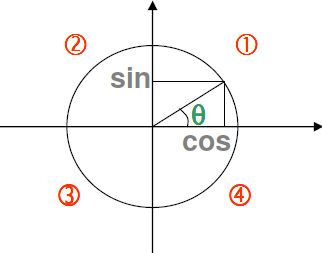
\includegraphics[width=4cm]{./bilder/einheitskreis.png}
    \end{minipage}






	\begin{minipage}{4cm}
    	\vspace{8mm}
    	$\theta=arctan2(\overbrace{y}^{sin},\overbrace{x}^{cos}) \Leftrightarrow$
    \end{minipage}
	\begin{minipage}[t]{0.8cm}
    	\textcircled{1}\\
    	\textcircled{2}\\
    	\textcircled{3}\\
    	\textcircled{4}
    \end{minipage}
	\begin{minipage}[t]{3.5cm}
    	$\theta= arctan(\frac{y}{x})$\\
    	$\theta= \pi + arctan(\frac{y}{x})$\\
    	$\theta= -\pi + arctan(\frac{y}{x})$\\
    	$\theta= -arctan(\frac{y}{x})$\\
    \end{minipage}
	\begin{minipage}[t]{2.5cm}
    	\hspace{2mm} $0 \leq \theta \leq \frac{\pi}{2}$\\
    	\hspace*{1.5mm} $\frac{\pi}{2} \leq \theta \leq \pi$\\
    	$-\pi \leq \theta \leq -\frac{\pi}{2}$\\
    	$-\frac{\pi}{2} \leq \theta \leq 0$
    \end{minipage}
	\begin{minipage}[t]{2.5cm}
    	für $+y$, $+x$\\
    	für $+y$, $-x$\\
    	für $-y$, $-x$\\
    	für $-y$, $+x$
    \end{minipage}
	\begin{minipage}[t]{4cm}
     	\begin{tabular}[t]{|l}
    	$\theta = \frac{\pi}{2}$ für $x=0$, $y>0$\\
    	$\theta = - \frac{\pi}{2}$ für $x=0$, $y<0$\\
    	$\theta = 0$ für $x=0$, $y=0$\\
    	\end{tabular}
    \end{minipage}

$Arctan2$ mit TR: \texttt{$R \blacktriangleright P \theta (X,Y)$}
\hspace{2cm} {\color{red} ACHTUNG: X und Y sind vertauscht!!!}


\subsection{Rücktransformation auf Winkel}
	\begin{minipage}{9.5cm}
    	\begin{tabular}{|p{2.5cm}|p{6cm}|}
        \hline
        	\multicolumn{2}{|l|}{\textbf{Raumfestes Koordinatensystem}}\\
        	\multicolumn{2}{|l|}{(X-Y-Z Roll-Gier-Nick Winkel)}\\
        \hline
    		Rotationsmatrix:
    		& ${^A_B}R(\alpha,\beta,\gamma) = 
    			\begin{bmatrix} 
			    	r_{11} & r_{12} & r_{13} \\
			        r_{21} & r_{22} & r_{23} \\
			        r_{31} & r_{32} & r_{33}                              
			    \end{bmatrix}$ \\
		\hline
			Ansatz:
			& $cos\beta = \sqrt{r^2_{11} + r^2_{21}}$ \\
			& $sin\beta = -r_{31}$\\
		\hline
			Winkel:
			& $\beta=arctan2(-r_{31},\sqrt{r^2_{11}+r^2_{21}})$\\
			& $\alpha=arctan2(\frac{r_{21}}{cos\beta},\frac{r_{11}}{cos\beta})$\\
			& $\gamma=arctan2(\frac{r_{32}}{cos\beta},\frac{r_{33}}{cos\beta})$\\
		\hline
			wenn $\beta=90^{\circ}$:
			& $\alpha=0^{\circ},\gamma=arctan2(r_{12},r_{22})$\\
			wenn $\beta=-90^{\circ}$:
			& $\alpha=0^{\circ},\gamma=-arctan2(r_{12},r_{22})$\\
		\hline
        \end{tabular}
    	
    \end{minipage}
	\begin{minipage}{9.5cm}
    	\begin{tabular}{|p{2.5cm}|p{6cm}|}
        \hline
        	\multicolumn{2}{|l|}{\textbf{Körperfestes Koordinatensystem}}\\
        	\multicolumn{2}{|l|}{(Z-Y-Z Euler Winkel)}\\
        \hline
        	Rotationsmatrix:
    		& ${^A_B}R(\alpha,\beta,\gamma) = 
    			\begin{bmatrix} 
			    	r_{11} & r_{12} & r_{13} \\
			        r_{21} & r_{22} & r_{23} \\
			        r_{31} & r_{32} & r_{33}                              
			    \end{bmatrix}$ \\
		\hline
			Ansatz:
			& $sin\beta = \sqrt{r^2_{31} + r^2_{32}}$ \\
			& $cos\beta = r_{33}$\\
		\hline
			Winkel:
			& $\beta=arctan2(\sqrt{r^2_{31}+r^2_{32}},r_{33})$\\
			& $\alpha=arctan2(\frac{r_{23}}{sin\beta},\frac{r_{13}}{sin\beta})$\\
			& $\gamma=arctan2(\frac{r_{32}}{sin\beta},\frac{r_{31}}{sin\beta})$\\
		\hline
			wenn $\beta=0^{\circ}$:
			& $\alpha=0^{\circ},\gamma=arctan2(-r_{12},r_{11})$\\
			wenn $\beta=180^{\circ}$:
			& $\alpha=0^{\circ},\gamma=-arctan2(r_{12},-r_{11})$\\
		\hline
        \end{tabular}
    	

    	
    \end{minipage}
	
	\newpage
	\subsection{Transformations Matrix}
	\subsubsection{Aufbau \small{ (RotationsMatrix und Verschiebung in einer
	Matrix)}}
		\begin{minipage}{10cm}
			Transformationsmatrix: T = $ 
    			\begin{bmatrix} 
			    	r_{11} & r_{12} & r_{13} & o_{ab} \\
			        r_{21} & r_{22} & r_{23} & o_{ab} \\
			        r_{21} & r_{22} & r_{23} & o_{ab} \\
			        0 & 0 & 0 & x                              
			    \end{bmatrix}$
		\end{minipage}
		\begin{minipage}{10cm}
    			x = 1 bei Ortsvektor \\
				x = 0 bei Feiem Vektor
		\end{minipage}
	\subsubsection{Multiplikation}
		Transformations Matrix über mehrere Koordinatensysteme:\\
		
		${}^0_n\mathrm{T}={}^0_1\mathrm{T}\cdot{}^1_2\mathrm{T}\cdot{}$\ldots$\cdot{}^{n-1}_n\mathrm{T}$;
		\space\space\space\space ${}^A_B\mathrm{T} \Rightarrow$
		Transformationsmatrix von Koordinatensystem A nach B
    	
	\subsubsection{Punkte in verschiedenen Koordinatensystemen}
		${}^B\mathrm{P}={}^B_A\mathrm{T}\cdot{}^A\mathrm{P}$ \\ \\
		${}^A\mathrm{P}={}^B_A\mathrm{T}^{-1}\cdot{}^B\mathrm{P}$
		
		
		

	\subsection{Jacobi Matrix \small{ (erklärt durch Beispiel)}}
		
		
        Die Jacobi-Matrix eines Roboterarms beschreibt die Abbildung von
        Gelenkgeschwindigkeiten auf die Lineargeschwindigkeit des TCP
        und die zeitlichen Änderungen der Orientierung des End-Effektors
        bezogen auf ein Referenzkoordinatensystemk z.B. auf das
        Basiskoordinatensystem O auf. \\
        In der Positionsbeschreibung werden alle Parameter die einen Einfluss 
       auf den Greifer haben aufgestellt und dann für die Jakobi-Matrix nach diesen Partiell abgeleitet. \\
    
	     \begin{minipage}{5cm}
	        Für die Jacobi Matrizen \\
	        empfehlen sich \\
	        Kurzschreibweisen
	        \end{minipage}
			\begin{minipage} {8cm}
            
	        $ c_{12}=cos(\theta_{1} + \theta_{2}) $ \\
	        $ s_{12}=sin(\theta_{1} + \theta_{2}) $
	        
	        \end{minipage}\\ \\
	     \begin{minipage}{12cm}
	     \subsubsection{Vorwärtskinematik}
	     	Geg: Gelenkkoordinaten und Geschwindigkeiten: $q ; \dot{x}$ \\
			Ges: Geschwindigkeit des Endeffektors: $\dot{X} = [\dot{x} \dot{y} \dot{z}
			\dot{\alpha} \dot{\beta} \dot{\gamma}]^{T}$ \\ 
			Lsg: Jacobi-Matrix $ \Longrightarrow \dot{X}=J(q)*\dot{q}$ \\ \\
			Positionsbeschreibung des Endeffektors: \\
	     $
	    			\begin{bmatrix} 
				    	x_{e} \\
				        y_{e} \\                             
				    \end{bmatrix}
					=
					\begin{bmatrix} 
				    	d_{2}cos\theta_{1}+l_{3}cos(\theta_{1}+\theta_{3}) \\
				        d_{2}sin\theta_{1}+l_{3}sin(\theta_{1}+\theta_{3}) \\                              
				    \end{bmatrix} $ und $ \Phi_{e}=\theta_{1}+\theta_{3} \\ \\$
			Jacobi-Matrix: \\ $
				J = 
					\begin{bmatrix} 
				    	\frac{\partial{x_{e}}}{\partial{\theta_{1}}} & 
				    	\frac{\partial{x_{e}}}{\partial{d_{2}}} & 
				    	\frac{\partial{x_{e}}}{\partial{\theta_{3}}} \\
				    	\frac{\partial{y_{e}}}{\partial{\theta_{1}}} & 
				    	\frac{\partial{y_{e}}}{\partial{d_{2}}} & 
				    	\frac{\partial{y_{e}}}{\partial{\theta_{3}}} \\
				    	\frac{\partial{\Phi_{e}}}{\partial{\theta_{1}}} & 
				    	\frac{\partial{\Phi_{e}}}{\partial{d_{2}}} & 
				    	\frac{\partial{\Phi_{e}}}{\partial{\theta_{3}}} \\ 
				    \end{bmatrix} \\
			$ \space  $	=
					\begin{bmatrix} 
					    	-d_{2}sin(\theta_{1})-l_{3}sin(\theta_{1}+\theta_{3}) & 
					    	cos(\theta_{1}) & 
					    	-l_{3}sin(\theta_{1}+\theta_{3}) \\
					        d_{2}cos(\theta_{1})+l_{3}cos(\theta_{1}+\theta_{3}) & 
					        sin(\theta_{1}) & 
					        l_{3}cos(\theta_{1}+\theta_{3}) \\
					        1 & 
					        0 & 
					        1 \\                            
					    \end{bmatrix}$		
			\end{minipage}
			\begin{minipage}{8cm}
			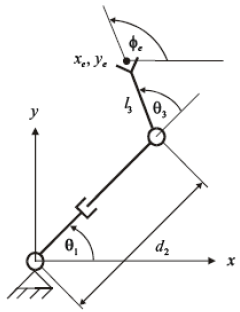
\includegraphics[width=5cm]{./bilder/jacobi-bsp.png}
			\end{minipage}
			
			\subsubsection{Rückwertskinematik}
			Geg: Geschwindigkeiten des Endeffektors: $\dot{x}$ \\
			Ges: Gelenkgeschwindigkeiten: $\dot{q}$ \\
			Lsg: Jacobi-Matrix $ \Longrightarrow \dot{q}=J^{-1}\dot{x}$ \\ \\
			Singularität: \\
			Die Jacobi-Matrix kann in singulären Stellungen
			nicht invertiert werden (d.h. die Determinante von J ist 0) und der Roboter
			kann in bestimmten Richtungen keine Bewegungen
			vornehmen. \\
			Mehr: Skript-Kinematik (S.11 ff) \& UB5 Bahnplanung (Aufg. 2))
			
\subsection{Denavit-Hartenberg}
\begin{minipage}{19cm}
	\textbf{Ablauf:}
	\begin{enumerate}{\setlength{\itemsep}{0cm}\setlength{\parsep}{0cm} \setlength{\topsep}{0cm}}
      \item Gelenke nummerieren in aufsteigender Reihenfolge. Starten in der Basis mit Nummer null.
      \item Jeden Achskörper mit Koordinatensystem belegen.
      \item Die $z_i$-Koordinatenachse muss mit der i+1 Gelenkachse zusammenfallen.
      \item Die $x_i$-Achse liegt entlang der Normalen zwischen der $z_{i-1}$ und $z_i$-Achse und zeigt vom Gelenk i zum Gelenk i+1.
      \item $y_i$-Achsen vervollständigen mit der Rechten-Hand-Regel. (x:Daumen, y:Zeigfinger, z:Mittelfinger)
      \item Festlegen der DH-Parameter (siehe DH-Parameter) und eintragen in DH-Tabelle.
      \item DH-Matrizen berechnen und miteinander mulitplizieren.
    \end{enumerate}
    \vspace{0.2cm}
\end{minipage}\\

\begin{minipage}{19cm}
	\textbf{Anmerkung Koordinatensysteme:}
	\begin{itemize}\itemsep0pt
      \item $z_i$-Achse muss grundsätzlich mit Bewegungsachse des zugehörigen Achskörper zusammenfallen.
      		Bei Rotationsgelenken gilt die Rechte-Handregel für Drehungen. 
      \item Ursprung des Koordinatensystems im Schnittpunkt der Bewegungsachsen.
    \end{itemize}
    \vspace{0.2cm}
\end{minipage}\\

\begin{minipage}{19cm}
	\textbf{DH-Parameter:}\\ \\
	\begin{tabular}{l l}
  		Linklänge $a_i$ (Fixwert): 				& Für $z_{i-1}$- und $z_i$-Achse wird die gem. Normale mit Länge $a_i$ in $x_i$-Richtung gemessen.\\
  		Linkdrehung $\alpha_{i}$ (Fixwert):		& Drehwinkel um $x_i$-Achse bis $z_{i-1}$- und $z_i$-Achse in gleiche Richtung zeigen.\\
  		Link Offset $d_i$ (Variable):			& Abstand von $x_{i-1}$- und $x_i$-Achse entlang der $z_{i-1}$-Achse.\\
 	 	Gelenkwinkel $\theta_{i}$ (Variable):	& Drehwinkel um $z_{i-1}$-Achse bis $x_{i-1}$- und $x_i$-Achse in gleiche Richtung zeigen.\\
    \end{tabular}
	\vspace{0.5cm}
\end{minipage}\\
\begin{minipage}{19cm}
\textbf{DH-Tabelle:}\\ \\
	\begin{minipage}{10cm}
    	\renewcommand{\arraystretch}{1.1}
			\begin{tabular}{| c | c | c | c | c |}
				\hline
					\textbf{Gelenk Nr.}
					& \textbf{Linklänge $a_i$}
					& \textbf{Linkdrehung $\alpha_{i}$}
					& \textbf{Link Offset $d_i$} 
					& \textbf{Gelenkwinkel $\theta_{i}$}\\
				\hline
					i
					&&&& \\
				\hline
					i+1
					&&&& \\
				\hline
					\ldots
					&&&&\\
				\hline
			\end{tabular}
		\renewcommand{\arraystretch}{1}
		\vspace{0.5cm}
    \end{minipage}
\end{minipage}\\
\begin{minipage}{19cm}
	\textbf{DH-Matrizen:}\\ \\
	$ ^{i-1}_{i}T =
	\begin{bmatrix}
    	cos(\theta_i) & -sin(\theta_i) cos(\alpha_i) &  sin(\theta_i) sin(\alpha_i) & a_i cos(\theta_i)\\
    	sin(\theta_i) &  cos(\theta_i) cos(\alpha_i) & -cos(\theta_i) sin(\alpha_i) & a_i sin(\theta_i)\\
    	0			  &  sin(\alpha_i)				 &  cos(\alpha_i)				& d_i\\
    	0			  &  0							 &  0							& 1\\
    \end{bmatrix}
\qquad
	 ^{0}_{n}T = \prod\limits_{i=1}^{n} \quad ^{i-1}_{i}T(\theta_{i}) = ^{0}_{1}T \cdot ^{1}_{2}T \cdot \ldots \cdot ^{n-1}_{n}T $
\end{minipage}\\\\

\begin{minipage}{3cm}
\textbf{Beispiel:}
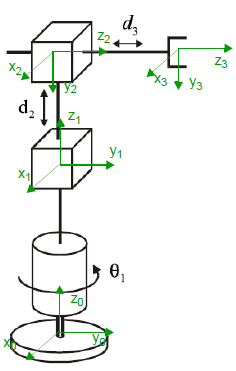
\includegraphics[width=4cm]{./bilder/denavit_grafik.png} \\
\end{minipage}
\begin{minipage}{6cm}
$\alpha_{i} \Longrightarrow $ Linkdrehung  \\
$ a_{i} \Longrightarrow $ Linklänge [Achsenabstand] \\
$ d_{i} \Longrightarrow $ Offset \\
$ \Theta_{i} \Longrightarrow $ Gelenkwinkel \\ 
\end{minipage}
\begin{minipage}{8cm}
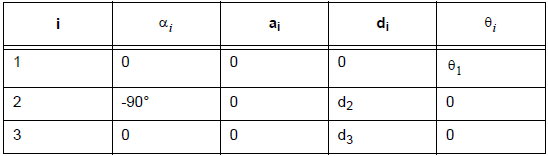
\includegraphics[width=9cm]{./bilder/denavit_tabelle.png} \\
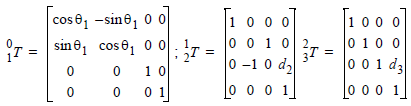
\includegraphics[width=9cm]{./bilder/denavit_matrix.png} \\
\end{minipage} \\





\newpage

\section{Kinematik, Kräfte \& Dynamik}
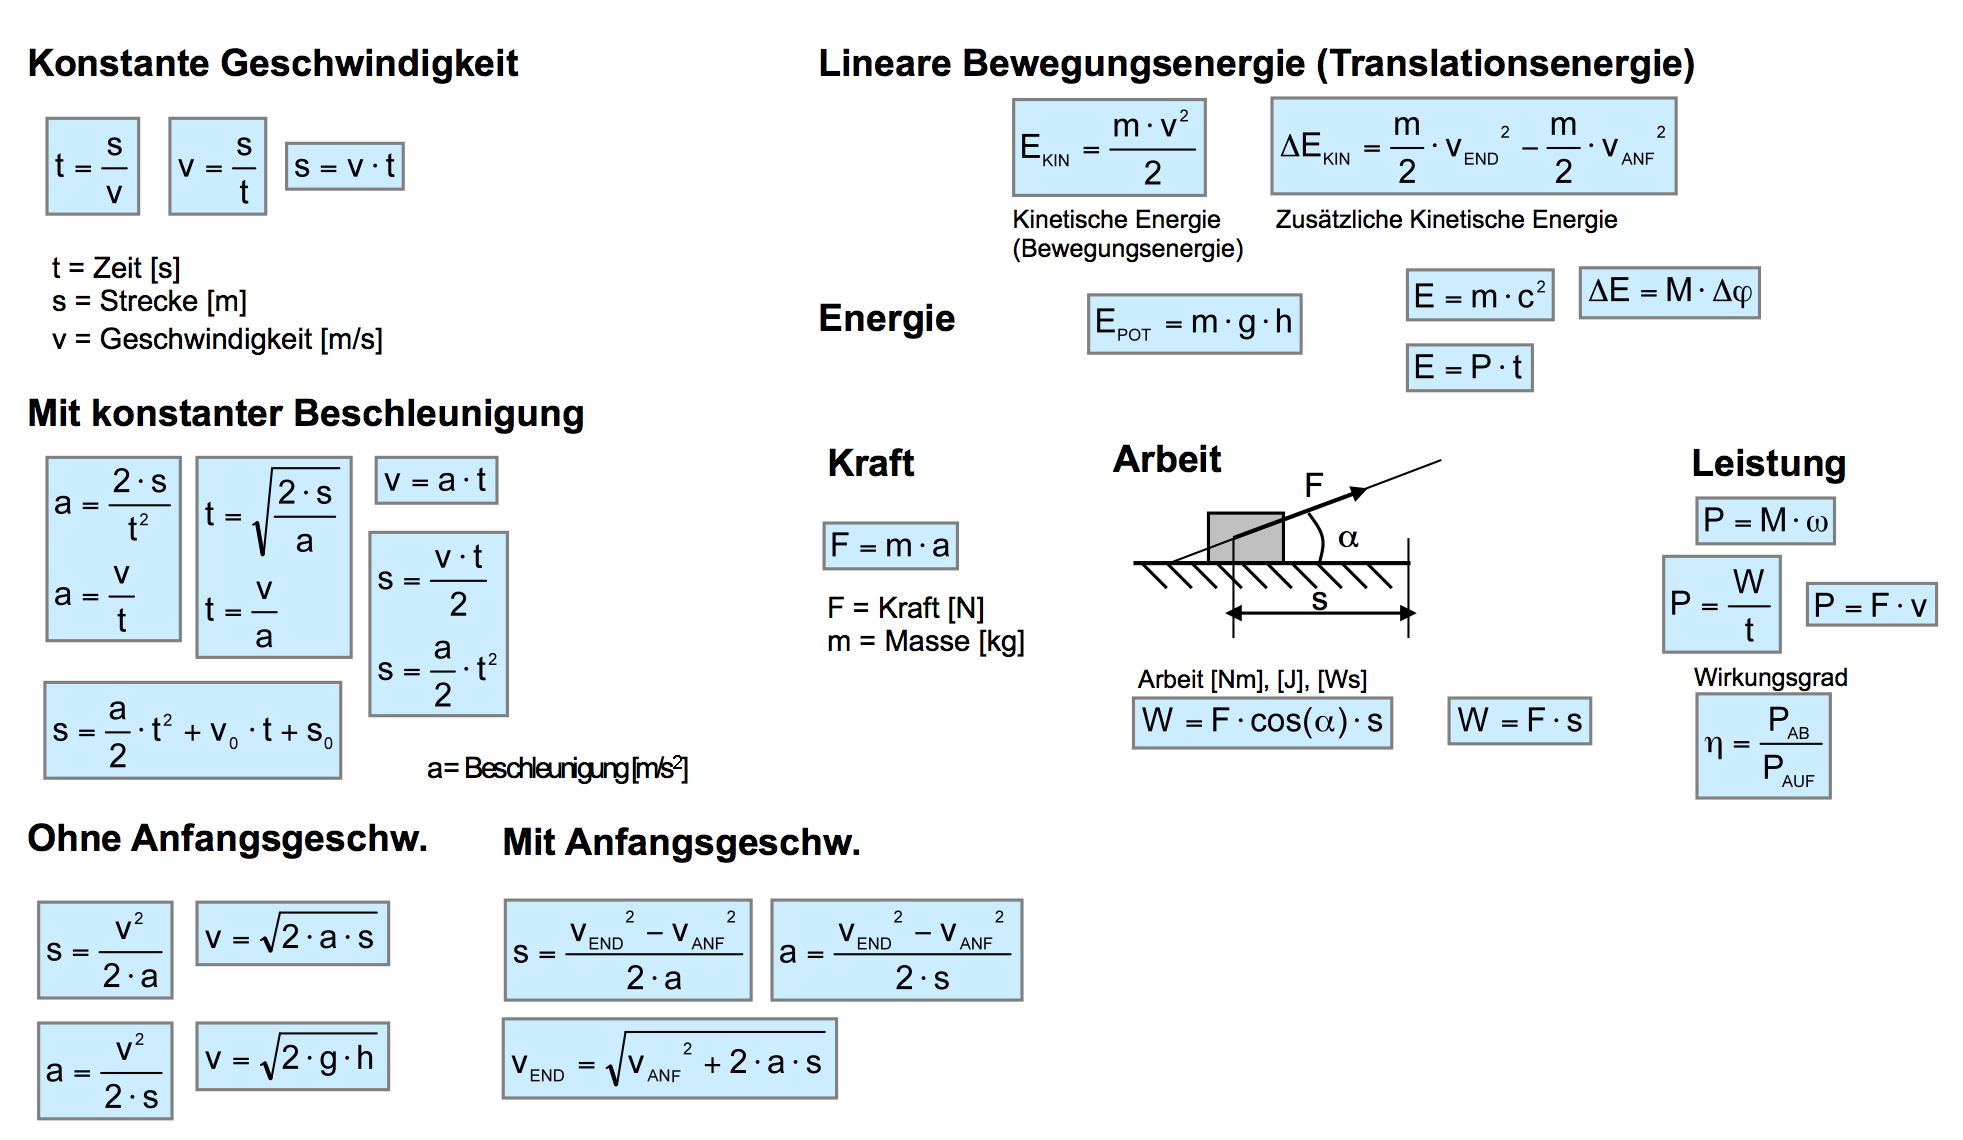
\includegraphics[width=17cm]{./bilder/kinematik.png} \\

\subsection{Kräfte}
$\tau_{n}={}^0J^T_n \cdot {}^0F_n  \\ \\
{}^0F_n = \begin{bmatrix} {}^0F_{x,n} & {}^0F_{y,n} & {}^0F_{z,n} & {}^0M_{x,n}
& {}^0M_{y,n} & {}^0M_{z,n}
\end{bmatrix}^{T}  \\ \\
zum Beispiel: \\
\begin{bmatrix}
\tau_{1} \\ \tau_{2} \\ \tau_{3}
\end{bmatrix}          
=  J \cdot
\begin{bmatrix}
F_{x} \\ F_{y} \\ F_{z}
\end{bmatrix}
$


\newpage

\section{Wichtige Formeln}
	$\sin^2(b)+\cos^2(b)=1 \qquad \tan(b)=\frac{\sin(b)}{\cos(b)}$

\subsection{Funktionswerte für Winkelargumente}
	\renewcommand{\arraystretch}{1.5}
	\begin{minipage}{5cm}
		\begin{tabular}[c]{ |c|c||c|c|c| }
	    	\hline
			deg & rad & sin & cos & tan\\
			\hline
			0\symbol{23} & 0 & 0 & 1 & 0\\
			\hline
			30\symbol{23} & $\frac{\pi}{6}$ & $\frac{1}{2}$ & $\frac{\sqrt{3}}{2}$ &
			$\frac{\sqrt{3}}{3}$\\
			\hline
			45\symbol{23} & $\frac{\pi}{4}$ & $\frac{\sqrt{2}}{2}$ & $\frac{\sqrt{2}}{2}$
			& 1\\
			\hline
			60\symbol{23} & $\frac{\pi}{3}$ & $\frac{\sqrt{3}}{2}$ & $\frac{1}{2}$ &
			$\sqrt{3}$\\
			\hline			
		\end{tabular}			
	\end{minipage}
	\begin{minipage}{4.3cm}
		\begin{tabular}[c]{ |c|c||c|c|}
	    	\hline
			deg & rad & sin & cos\\
			\hline
			90\symbol{23} & $\frac{\pi}{2}$ & 1 & 0\\
			\hline	
			120\symbol{23} & $\frac{2\pi}{3}$ & $\frac{\sqrt{3}}{2}$ & $-\frac{1}{2}$ \\
			\hline
			135\symbol{23} & $\frac{3\pi}{4}$ & $\frac{\sqrt{2}}{2}$ & $-\frac{\sqrt{2}}{2}$\\
			\hline
			150\symbol{23} & $\frac{5\pi}{6}$ & $\frac{1}{2}$ & $-\frac{\sqrt{3}}{2}$\\
			\hline
		\end{tabular}			
	\end{minipage}
	\begin{minipage}{4.5cm}
		\begin{tabular}[c]{ |c|c||c|c| }
	    	\hline
			deg & rad & sin & cos\\
			\hline
			180\symbol{23} & $\pi$ & 0 & -1\\
			\hline	
			210\symbol{23} & $\frac{7\pi}{6}$ & $-\frac{1}{2}$ & $-\frac{\sqrt{3}}{2}$\\
			\hline
			225\symbol{23} & $\frac{5\pi}{4}$ & $-\frac{\sqrt{2}}{2}$ & $-\frac{\sqrt{2}}{2}$\\
			\hline
			240\symbol{23} & $\frac{4\pi}{3}$ & $-\frac{\sqrt{3}}{2}$ & $-\frac{1}{2}$\\
			\hline
		\end{tabular}			
	\end{minipage}
	\begin{minipage}{4.5cm}
		\begin{tabular}[c]{ |c|c||c|c| }
	    	\hline
			deg & rad & sin & cos\\
			\hline
			270\symbol{23} & $\frac{3\pi}{2}$ & -1 & 0\\
			\hline	
			300\symbol{23} & $\frac{5\pi}{3}$ & $-\frac{\sqrt{3}}{2}$ & $\frac{1}{2}$\\
			\hline
			315\symbol{23} & $\frac{7\pi}{4}$ & $-\frac{\sqrt{2}}{2}$ & $\frac{\sqrt{2}}{2}$\\
			\hline
			330\symbol{23} & $\frac{11\pi}{6}$ & $-\frac{1}{2}$ & $\frac{\sqrt{3}}{2}$\\
			\hline
		\end{tabular}			
	\end{minipage}
	\renewcommand{\arraystretch}{1}
	
	\subsection{Periodizität}
	$\cos(a+k\cdot2\pi)=\cos(a) \qquad \sin(a+k\cdot2\pi)=\sin(a) \qquad
	(k \in \mathbb{Z})$
	
\subsection{Quadrantenbeziehungen}
	\begin{tabbing}
     	xxxxxxxxxxxxxxxxxxxxxxxxxxxxxxxxxx \= \kill
	  	$\sin(-a)=-\sin(a)$ \> $\cos(-a)=\cos(a)$\\
		$\sin(\pi - a)=\sin(a)$ \> $\cos(\pi - a)=-\cos(a)$\\
		$\sin(\pi + a)=-\sin(a)$ \> $\cos(\pi +a)=-\cos(a)$\\
		$\sin\left(\frac{\pi}{2}-a \right)=\sin\left(\frac{\pi}{2}+a \right)=\cos(a)$ \>
		$\cos\left(\frac{\pi}{2}-a \right)=-\cos\left(\frac{\pi}{2}+a \right)=\sin(a)$  
    \end{tabbing}


\begin{minipage}{12.5cm}
	\subsection{Additionstheoreme}
		$\sin(a \pm b)=\sin(a) \cdot \cos(b) \pm \cos(a) \cdot \sin(b)$\\
		$\cos(a \pm b)=\cos(a) \cdot \cos(b) \mp \sin(a) \cdot \sin(b)$\\	
		$\tan(a \pm b)=\frac{\tan(a) \pm \tan(b)}{1 \mp \tan(a) \cdot \tan(b)}$
		
	\subsection{Doppel- und Halbwinkel}	
		$\sin(2a)=2\sin(a)\cos(a)$\\
		$\cos(2a)=\cos^2(a)-\sin^2(a)=2\cos^2(a)-1=1-2\sin^2(a)$\\
		$\cos^2 \left(\frac{a}{2}\right)=\frac{1+\cos(a)}{2} \qquad
		\sin^2 \left(\frac{a}{2}\right)=\frac{1-\cos(a)}{2}$ \\ 
	\subsection{Summe, Differenz und Produkte}
	\begin{minipage}{7.5cm}	
		$\sin(a)+\sin(b)=2 \cdot \sin \left(\frac{a+b}{2}\right) \cdot
		\cos\left(\frac{a-b}{2}\right)$\\
		$\sin(a)-\sin(b)=2 \cdot \sin \left(\frac{a-b}{2}\right) \cdot
		\cos\left(\frac{a+b}{2}\right)$\\
		$\cos(a)+\cos(b)=2 \cdot \cos \left(\frac{a+b}{2}\right) \cdot
		\cos\left(\frac{a-b}{2}\right)$\\
		$\cos(a)-\cos(b)=-2 \cdot \sin \left(\frac{a+b}{2}\right) \cdot
		\cos\left(\frac{a-b}{2}\right)$\\
		$\tan(a) \pm \tan(b)=\frac{\sin(a \pm b)}{\cos(a)\cos(b)}$	\\
	\end{minipage}
	\begin{minipage}{6cm}
		$\sin(a)\sin(b)=\frac{1}{2}(\cos(a-b)-cos(a+b))$\\
		$\cos(a)\cos(b)=\frac{1}{2}(\cos(a-b)+cos(a+b))$\\
		$\sin(a)\cos(b)=\frac{1}{2}(\sin(a-b)+\sin(a+b))$\\
	\end{minipage}	
	
	\subsection{Differentialrechnung}
	\begin{minipage}{5cm}
    $ a \Longrightarrow 0$ \space $[a=const.]\\
    x \Longrightarrow 1 \\
    sin(x)\Longrightarrow cos(x) \\
    cos(x)\Longrightarrow -sin(x) \\
    tan(x)\Longrightarrow \frac{1}{cos^{2}(x)} \\
    $
    \end{minipage}
	\begin{minipage}{6cm}
    $ (u+v-w)' = u'+v'-u' \\
    (au)'= au'$ \space $ [a=const.]\\
    (uv)'=u'v + uv' \\
    (\frac{u}{v})' = \frac{vu'-uv'}{v^{2}} \\
    (u(v(y(x))))' = u'(v)v'(y)y'(x) \\
    $
    \end{minipage}
    	
\end{minipage}


\newpage

\section{Symbole und Theorie}
	\subsection{Darstellung kinematischer Gelenke}
		
		\begin{minipage}{10cm}
		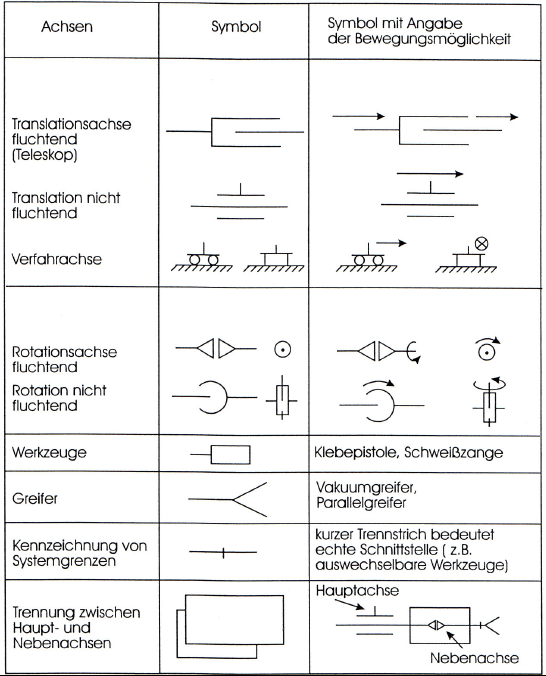
\includegraphics[width=10cm]{./bilder/symbole.png}
		\end{minipage}
		\begin{minipage}{8cm}
		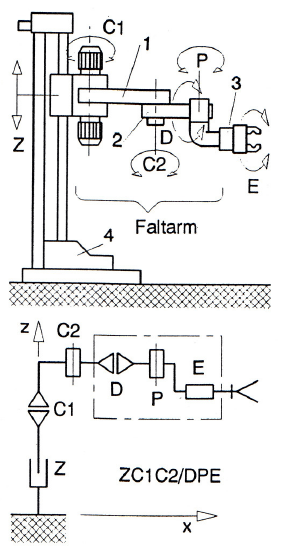
\includegraphics[width=5cm]{./bilder/symbole-bsp.png}
		\end{minipage}

	\subsection{Bewegungsarten}
		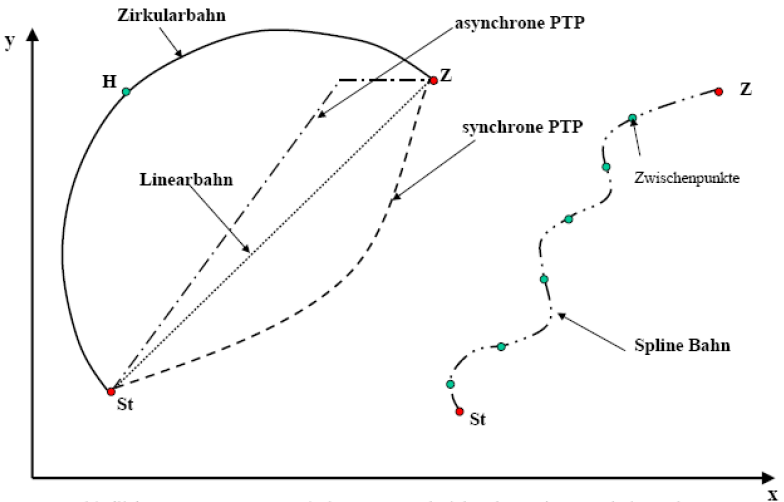
\includegraphics[width=10cm]{./bilder/bewegungsarten.png}
	
	\subsection{PTP-Synchron}
	\begin{minipage}{6cm}
		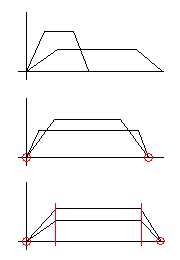
\includegraphics[width=5cm]{./bilder/synchron.png}
    \end{minipage}
	\begin{minipage}{12.5cm}
    	Asynchron PTP\\ \\ \\ \\ \\ \\
    	Synchron PTP\\ \\ \\ \\ \\ \\
    	Vollsynchron PTP\\
    \end{minipage}

	\subsection{Übersicht von Skript und Übungen}
	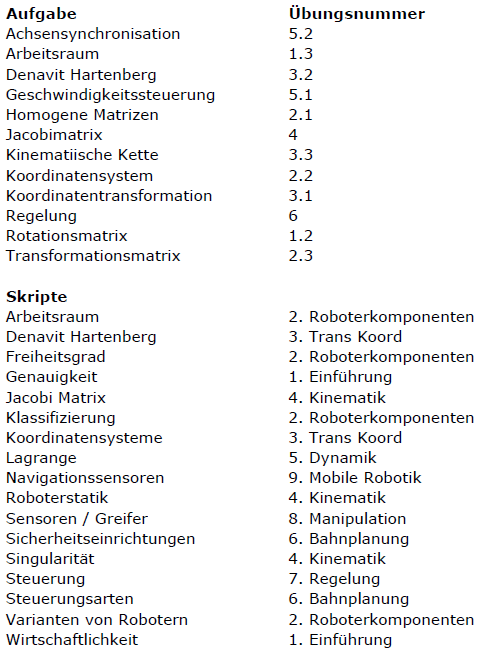
\includegraphics[width=10cm]{./bilder/uebersicht.png}



  
\end{document}
	

